%!TEX root = ../sbc-template.tex

As \emph{Smart} TVs são tidas como aparelhos de televisão com capacidades interativas ligadas à internet, como aplicativos disponíveis em lojas; acesso a conteúdo online como notícias, previsão do tempo, informações de mercados de ações, mapas e jogos; \emph{e-commerce}; navegação web e acesso a redes sociais. Estes aparelhos podem ser equipadas com câmeras e microfones embutidos, além de óculos 3D, como mostra a Figura \ref{fig:smart_samsung}. Estas televisões utilizam os mesmos sistemas operacionais e conjuntos de aplicativos que computadores comuns, o que as torna sucetíveis às mesmas falhas e ataques de segurança que outros dispositivos semelhates. Contudo, \emph{Smart} TVs que adotem o padrão de compartilhameto de mídia DLNA(Digital Living Network Alliance) podem exibir conteúdos como filmes, imagens, músicas e outros diretamente de outros dispositivos como computadores e smartphones que estejam conectados à mesma rede sem fio \cite{michele2014watch}, \cite{shin2013smart}, \cite{perakakis2015proposed}, \cite{whatisasmarttv}.

O grande diferencial de hardware entre \emph{Smart} TVs e as antigas tecnologias \emph{LED} e \emph{LCD} TV reside na conexão com a internet \cite{differencebetween}. Os modelos podem vir equipados com módulo WiFi ou Ethernet \cite{tomsguid:everythingsmart}. Além disso, \emph{Smart} TVs também são equipadas com um navegador web e suas aplicações são desenvolvidas em linguagens de programação ``suportadas'' por navegadores web \cite{mautilus:specificationsforsmart}. Muitos modelos vêm equipados com ferramentas de reconhecimento de voz, como a \emph{Alexa}, que possibilita funcionalidades como troca e busca de canais, controle de volume, etc. O controle de voz também deverá estar integrado com funções de ``casa inteligente'', como os \emph{Smart Home Hubs} \cite{tomsguid:everythingsmart}. As principais marcas de \emph{Smart} TVs incluem a Hisence, LG, Panasonic, Phillips. Samsung, Sharp, Sony, TCL, Toshiba e Vizio \cite{tomsguid:everythingsmart}.


\begin{figure}[t]
	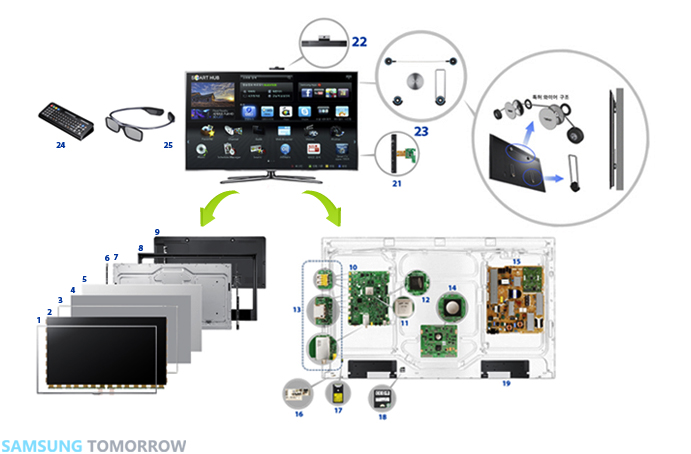
\includegraphics[width=\textwidth]{img/smart_samsung.jpg}
	\caption{Diagrama representativo de uma \emph{Smart} TV e seus componentes \cite{samsung:smarttv}}
	\label{fig:smart_samsung}
\end{figure}

\begin{table}[ht]
	\centering
	\caption{Legenda da Figura \ref{fig:smart_samsung}}
	\label{tab:smart}
	\begin{tabular}{c l}
		\hline
		Número & Descrição \\
		\hline
		1 & Moldura \\
		2 & Painel de cristal negro (célula) \\
		3 & Molde da moldura do meio \\
		4 & Folha óptica \\
		5 & LGP (Light Guide Plate) -- Prato guia leve \\
		6 & LED \\
		7 & Chassi traseiro \\
		8 & Cobertura do meio \\
		9 & Cobertura traseira \\
		10 & Placa de circuito principal (Placa mãe) \\
		11 & Smart Real Engine \\
		12 & Speed Backlite Engine \\
		13 & Sintonizador, 4 portas HDMI e 3 portas USB \\
		14 & 3D Hyper Real Engine \\
		15 & Placa de Alimentação \\
		16 & Sensor de luz ambiente \\
		17 & Módulo bluetooth \\
		18 & Módulo WiFi \\
		19 & Auto-falantes \\
		20 & Suporte quadrangular \\
		21 & Botão touch operacional \\
		22 & Câmera de video de telefone \\
		23 & Suporte de parede \\
		24 & Controle remoto QWERTY \\
		25 & Óculos 3D \\
		\hline
	\end{tabular}
\end{table}

A Figura \ref{fig:smart_samsung} exibe um diagrama representativo de uma \emph{Smart} TV. As legendas para os números apresentados na imagem estão na Tabela \ref{tab:smart}.

\begin{figure}[ht]
	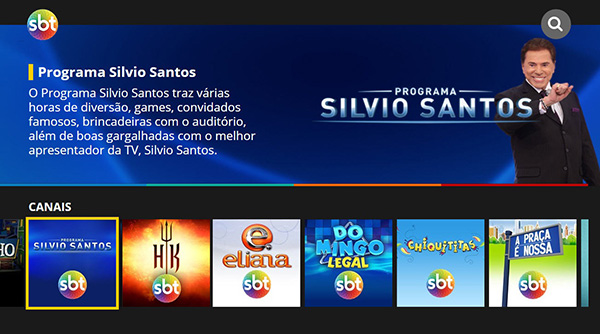
\includegraphics[width=\textwidth]{img/sbt_app.jpg}
	\caption{Aplicativo SBT. Fonte: \cite{sbt:tvconectada}}
	\label{fig:sbt_app}
\end{figure}

Um exemplo de aplicação desenvolvida para \emph{Smart} TVs é a disponibilizada desde 2016 pela emissora SBT. O aplicativo contém novelas, programas, entre outras partes da programação da emissora completos para ser assistidos on demand, como é mostrado na Figura \ref{fig:sbt_app} \cite{sbt:tvconectada}. Outros exemplos são os aplicativos de streaming como Netflix, Amazon Prime Video, Hulu e Pandora, ainda não disponíveis no Brasil; Crackle, Telecine Play, HBO Go, NetMovies, Globo Play, Google Play, iTunes Store, E! Plus, etc \cite{canaltech:streaming}.

Segundo a PNAD realizada pelo IBGE em 2015, 103 milhoes de televisões em residências e prontos comerciais, sendo 16 milhões Smart TV, 94$\%$ adquiridas entre 2014 e 2015 \cite{pnad2015}. No primeiro semestre de 2017 foram vendidos 5,22 milhões de televisões no Brasil, sendo $68,2\%$ deste total composto de Smart TVs. Este aumento é atribuido principalmente ao fim da transmissão de sinal analógico da televisão aberta \cite{leiajabuscasmart}, à Copa do Mundo 2018 e à tecnologia $4K$ \cite{correiopnad}.

Nota-se que o uso de Smart TVs está se diversificando. O consumidor pode escolher entre alternativas como serviços de streaming independente de provedores como Netflix, Google PLay e Globo Play, ou Hulu e Pandora(ainda não disponíveis no Brasil), ou alternativas como Crackle, Telecine Play e HBO Go, que requerem um provedor de serviços como Net, Claro ou Sky para que o usuário possa assinar o serviço. Há também as alternativas completamente online e gratuitas como YouTube e Facebook. Além disso, a transmissão de TV aberta digital aumenta a quantidade de canais captados gratuitamente por usuários, enquanto a qualidade de transmissão é HD, fazendo com que a tecnologia ainda seja a alternativa mais barata para o acesso de conteúdo em vídeo \cite{estadao:explosaovideosonline} \cite{tomsguid:everythingsmart}.
